% Options for packages loaded elsewhere
\PassOptionsToPackage{unicode}{hyperref}
\PassOptionsToPackage{hyphens}{url}
\PassOptionsToPackage{dvipsnames,svgnames,x11names}{xcolor}
%
\documentclass[
  ignorenonframetext,
  aspectratio=169,
]{beamer}
\usepackage{pgfpages}
\setbeamertemplate{caption}[numbered]
\setbeamertemplate{caption label separator}{: }
\setbeamercolor{caption name}{fg=normal text.fg}
\beamertemplatenavigationsymbolshorizontal
% Prevent slide breaks in the middle of a paragraph
\widowpenalties 1 10000
\raggedbottom
\setbeamertemplate{part page}{
  \centering
  \begin{beamercolorbox}[sep=16pt,center]{part title}
    \usebeamerfont{part title}\insertpart\par
  \end{beamercolorbox}
}
\setbeamertemplate{section page}{
  \centering
  \begin{beamercolorbox}[sep=12pt,center]{part title}
    \usebeamerfont{section title}\insertsection\par
  \end{beamercolorbox}
}
\setbeamertemplate{subsection page}{
  \centering
  \begin{beamercolorbox}[sep=8pt,center]{part title}
    \usebeamerfont{subsection title}\insertsubsection\par
  \end{beamercolorbox}
}
\AtBeginPart{
  \frame{\partpage}
}
\AtBeginSection{
  \ifbibliography
  \else
    \frame{\sectionpage}
  \fi
}
\AtBeginSubsection{
  \frame{\subsectionpage}
}

\usepackage{amsmath,amssymb}
\usepackage{iftex}
\ifPDFTeX
  \usepackage[T1]{fontenc}
  \usepackage[utf8]{inputenc}
  \usepackage{textcomp} % provide euro and other symbols
\else % if luatex or xetex
  \usepackage{unicode-math}
  \defaultfontfeatures{Scale=MatchLowercase}
  \defaultfontfeatures[\rmfamily]{Ligatures=TeX,Scale=1}
\fi
\usetheme[]{Hannover}
\usecolortheme{rose}
\usepackage[]{libertinus}
\ifPDFTeX\else  
    % xetex/luatex font selection
\fi
% Use upquote if available, for straight quotes in verbatim environments
\IfFileExists{upquote.sty}{\usepackage{upquote}}{}
\IfFileExists{microtype.sty}{% use microtype if available
  \usepackage[]{microtype}
  \UseMicrotypeSet[protrusion]{basicmath} % disable protrusion for tt fonts
}{}
\makeatletter
\@ifundefined{KOMAClassName}{% if non-KOMA class
  \IfFileExists{parskip.sty}{%
    \usepackage{parskip}
  }{% else
    \setlength{\parindent}{0pt}
    \setlength{\parskip}{6pt plus 2pt minus 1pt}}
}{% if KOMA class
  \KOMAoptions{parskip=half}}
\makeatother
\usepackage{xcolor}
\newif\ifbibliography
\setlength{\emergencystretch}{3em} % prevent overfull lines
\setcounter{secnumdepth}{-\maxdimen} % remove section numbering


\providecommand{\tightlist}{%
  \setlength{\itemsep}{0pt}\setlength{\parskip}{0pt}}\usepackage{longtable,booktabs,array}
\usepackage{calc} % for calculating minipage widths
\usepackage{caption}
% Make caption package work with longtable
\makeatletter
\def\fnum@table{\tablename~\thetable}
\makeatother
\usepackage{graphicx}
\makeatletter
\def\maxwidth{\ifdim\Gin@nat@width>\linewidth\linewidth\else\Gin@nat@width\fi}
\def\maxheight{\ifdim\Gin@nat@height>\textheight\textheight\else\Gin@nat@height\fi}
\makeatother
% Scale images if necessary, so that they will not overflow the page
% margins by default, and it is still possible to overwrite the defaults
% using explicit options in \includegraphics[width, height, ...]{}
\setkeys{Gin}{width=\maxwidth,height=\maxheight,keepaspectratio}
% Set default figure placement to htbp
\makeatletter
\def\fps@figure{htbp}
\makeatother

\makeatletter
\@ifpackageloaded{tcolorbox}{}{\usepackage[skins,breakable]{tcolorbox}}
\@ifpackageloaded{fontawesome5}{}{\usepackage{fontawesome5}}
\definecolor{quarto-callout-color}{HTML}{909090}
\definecolor{quarto-callout-note-color}{HTML}{0758E5}
\definecolor{quarto-callout-important-color}{HTML}{CC1914}
\definecolor{quarto-callout-warning-color}{HTML}{EB9113}
\definecolor{quarto-callout-tip-color}{HTML}{00A047}
\definecolor{quarto-callout-caution-color}{HTML}{FC5300}
\definecolor{quarto-callout-color-frame}{HTML}{acacac}
\definecolor{quarto-callout-note-color-frame}{HTML}{4582ec}
\definecolor{quarto-callout-important-color-frame}{HTML}{d9534f}
\definecolor{quarto-callout-warning-color-frame}{HTML}{f0ad4e}
\definecolor{quarto-callout-tip-color-frame}{HTML}{02b875}
\definecolor{quarto-callout-caution-color-frame}{HTML}{fd7e14}
\makeatother
\makeatletter
\@ifpackageloaded{caption}{}{\usepackage{caption}}
\AtBeginDocument{%
\ifdefined\contentsname
  \renewcommand*\contentsname{Table of contents}
\else
  \newcommand\contentsname{Table of contents}
\fi
\ifdefined\listfigurename
  \renewcommand*\listfigurename{List of Figures}
\else
  \newcommand\listfigurename{List of Figures}
\fi
\ifdefined\listtablename
  \renewcommand*\listtablename{List of Tables}
\else
  \newcommand\listtablename{List of Tables}
\fi
\ifdefined\figurename
  \renewcommand*\figurename{Figure}
\else
  \newcommand\figurename{Figure}
\fi
\ifdefined\tablename
  \renewcommand*\tablename{Table}
\else
  \newcommand\tablename{Table}
\fi
}
\@ifpackageloaded{float}{}{\usepackage{float}}
\floatstyle{ruled}
\@ifundefined{c@chapter}{\newfloat{codelisting}{h}{lop}}{\newfloat{codelisting}{h}{lop}[chapter]}
\floatname{codelisting}{Listing}
\newcommand*\listoflistings{\listof{codelisting}{List of Listings}}
\makeatother
\makeatletter
\makeatother
\makeatletter
\@ifpackageloaded{caption}{}{\usepackage{caption}}
\@ifpackageloaded{subcaption}{}{\usepackage{subcaption}}
\makeatother
\ifLuaTeX
  \usepackage{selnolig}  % disable illegal ligatures
\fi
\usepackage{bookmark}

\IfFileExists{xurl.sty}{\usepackage{xurl}}{} % add URL line breaks if available
\urlstyle{same} % disable monospaced font for URLs
\hypersetup{
  pdftitle={Quarto Crash Course},
  pdfauthor={Usman Afzali, PhD - Postdoctoral Fellow},
  colorlinks=true,
  linkcolor={Maroon},
  filecolor={Maroon},
  citecolor={Blue},
  urlcolor={Blue},
  pdfcreator={LaTeX via pandoc}}

\title{Quarto Crash Course}
\subtitle{For School of Psychology, Speech and Hearing}
\author{Usman Afzali, PhD - Postdoctoral Fellow}
\date{2024-07-18}
\institute{University of Canterbury}
\logo{
\includegraphics{mds.png}}

\begin{document}
\frame{\titlepage}

\begin{frame}
\begin{block}{Karakia Whakatūwhera}
\phantomsection\label{karakia-whakatux16bwhera}
\begin{figure}

\begin{minipage}{0.50\linewidth}
Whakataka te hau ki te uru/ Whakataka te hau ki te tonga/ Kia mākinakina
ki uta/ Kia mātaratara ki tai/ E hī ake ana te atakura/ He tio, he huka,
he hau hū/ Tīhei mauri ora!\end{minipage}%
%
\begin{minipage}{0.50\linewidth}
Cease the winds from the west/ Cease the winds from the south/ Let the
breeze blow over the land/ Let the breeze blow over the ocean/ Let the
red-tipped dawn come with a sharpened air./ A touch of frost, a promise
of a glorious day.\end{minipage}%

\end{figure}%
\end{block}
\end{frame}

\begin{frame}[fragile]{Kauhau}
\phantomsection\label{kauhau}
\begin{itemize}[<+->]
\tightlist
\item
  What is \texttt{Quarto}?
\item
  Documentation
\item
  Version control, Remote repositories, and Blogging
\item
  Templates
\item
  Presentation
\item
  Final thoughts
\end{itemize}

\begin{block}{Problem 1}
\phantomsection\label{problem-1}
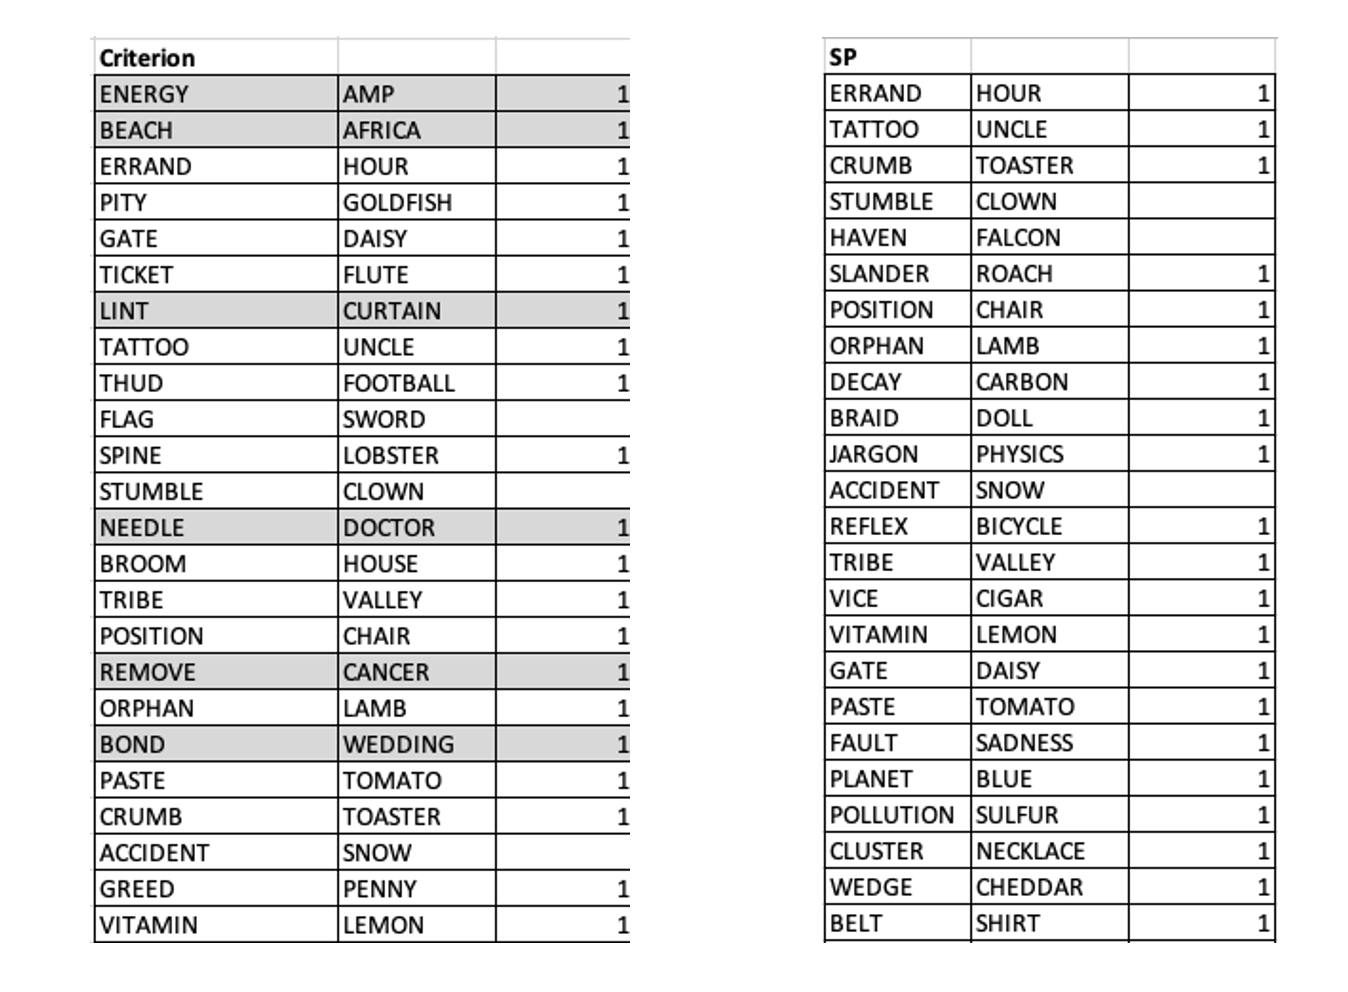
\includegraphics[width=0.7\textwidth,height=\textheight]{/posts/problem1.png}

\href{https://github.com/usman-afzali/think-no-think/blob/main/TNT-processing-code.py}{Solution}
\end{block}

\begin{block}{Problem(s) 2}
\phantomsection\label{problems-2}
\begin{itemize}
\tightlist
\item
  Time constraints and having to be efficient.
\item
  Having to redo a whole document only to change formatting for various
  purposes.
\item
  MS Word is not necessarily the best application for writing up.
\item
  The need to remember data analysis/stats decisions made along the way.
\end{itemize}

\begin{tcolorbox}[enhanced jigsaw, bottomrule=.15mm, breakable, colbacktitle=quarto-callout-important-color!10!white, left=2mm, toptitle=1mm, rightrule=.15mm, colback=white, coltitle=black, titlerule=0mm, title=\textcolor{quarto-callout-important-color}{\faExclamation}\hspace{0.5em}{What about the audience?}, opacityback=0, opacitybacktitle=0.6, colframe=quarto-callout-important-color-frame, toprule=.15mm, bottomtitle=1mm, arc=.35mm, leftrule=.75mm]

Any other similar problems?

\end{tcolorbox}
\end{block}

\begin{block}{My favourite(?!) problem}
\phantomsection\label{my-favourite-problem}

\includegraphics{/posts/final.jpeg}
\end{block}

\begin{block}{And then\ldots{}}
\phantomsection\label{and-then}

\includegraphics{/posts/mc-q.png}
\end{block}
\end{frame}

\begin{frame}[fragile]{Introduction}
\phantomsection\label{introduction}
\begin{block}{Quarto}
\phantomsection\label{quarto}
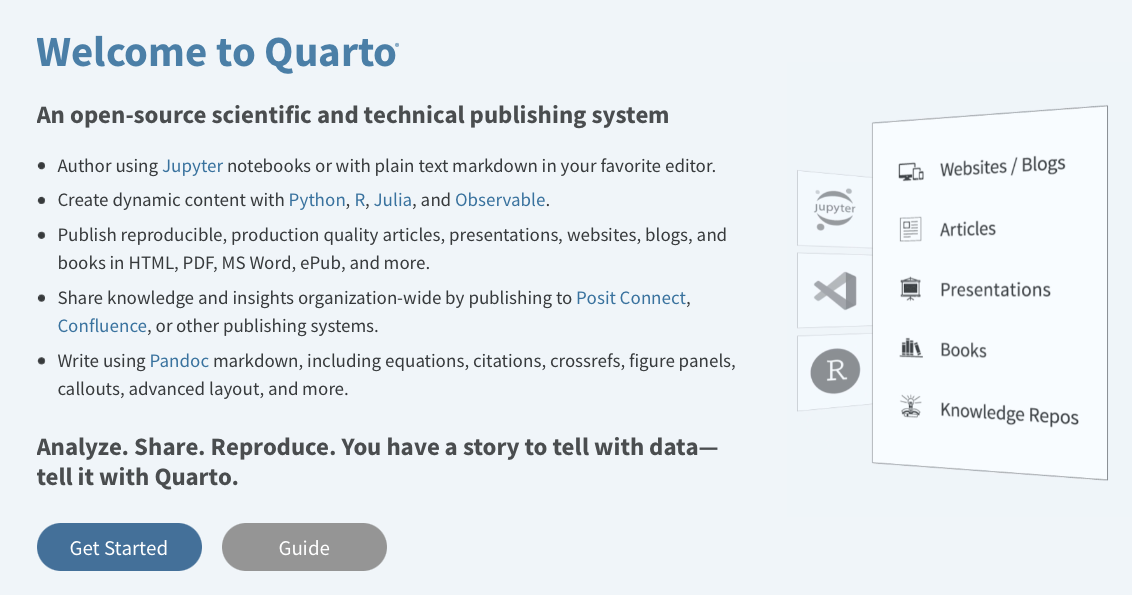
\includegraphics{/posts/quarto-intro.png}

\href{https://quarto.org}{Website}
\end{block}

\begin{block}{Featured in \emph{Nature}}
\phantomsection\label{featured-in-nature}
Cut the tyranny of copy-and-paste with these coding tools
{[}@perkel2022{]}

\begin{itemize}[<+->]
\tightlist
\item
  App-switching, updating your numbers, fix an error
\item
  Use \texttt{executable\ manuscripts}
\item
  ``Reduces the number of manual things you have to do'' (Sarah
  Pederzani)
\item
  Transparency
\item
  Version control
\item
  Collaboration
\item
  Steep curve :)
\end{itemize}
\end{block}
\end{frame}

\begin{frame}[fragile]{Documentation}
\phantomsection\label{documentation}
\begin{block}{Basics}
\phantomsection\label{basics}
\begin{itemize}[<+->]
\tightlist
\item
  Use the latest version of \texttt{RStudio}, at least
  \texttt{Version:\ 2022.12.0+353} or later on your computer.
\item
  Within \texttt{RStudio}, click on \texttt{new\ file} drop down menu
  and open a new \texttt{Quarto\ Document}, and name it.
  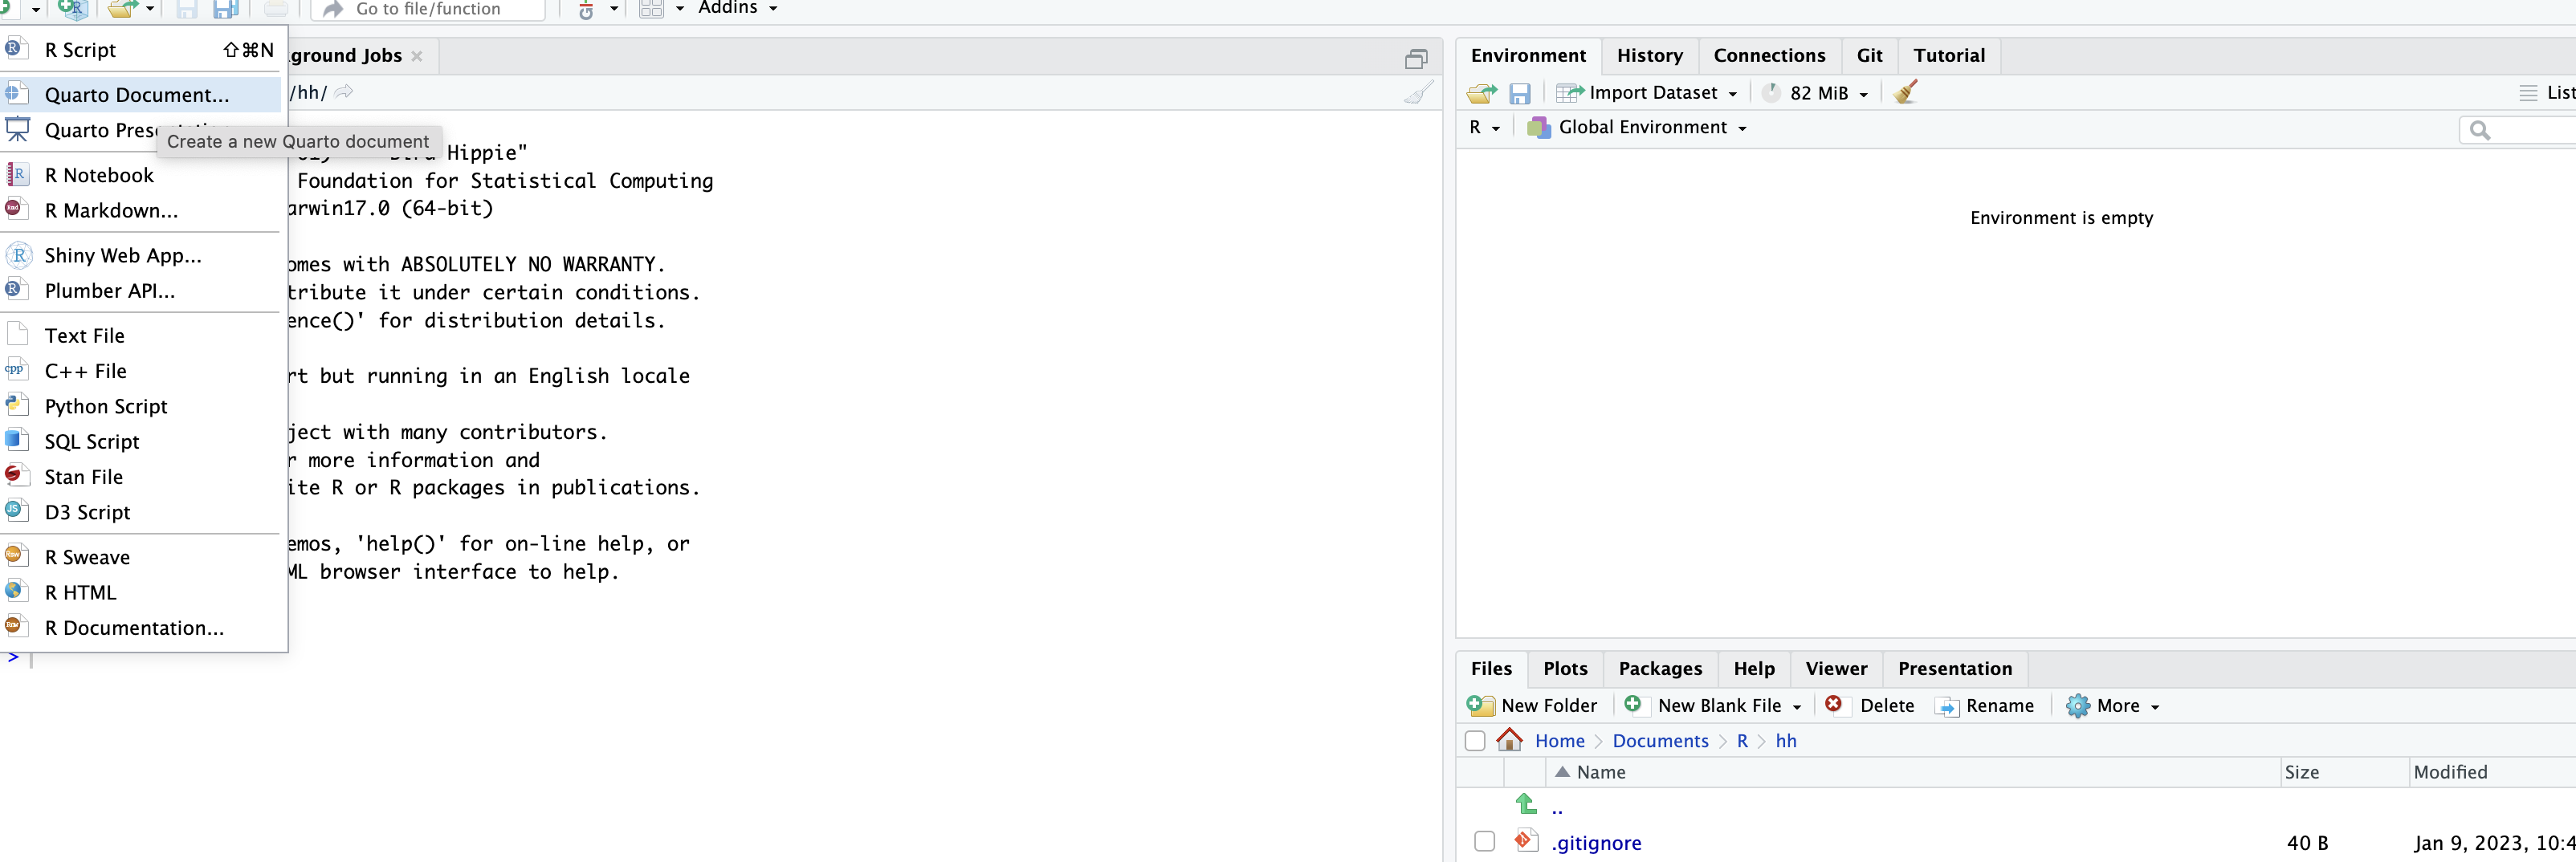
\includegraphics{/posts/r-interface.png}
\end{itemize}
\end{block}

\begin{block}{Basics cont\ldots{}}
\phantomsection\label{basics-cont}
\begin{itemize}
\tightlist
\item
  Let's have a sneak peak at different parts of a quarto document
  \href{https://monashdatafluency.github.io/r-rep-res-quarto/03-quarto-documents/index.html}{here}.
\item
  Once the \texttt{.qmd} document is opened, use either the
  \texttt{source} tab or \texttt{visual} tab to start documenting or
  writing code. Then hit \texttt{Render}. You will see output in the
  \texttt{Viewer} menu. See next slide.
\end{itemize}
\end{block}

\begin{block}{Basics cont\ldots{}}
\phantomsection\label{basics-cont-1}
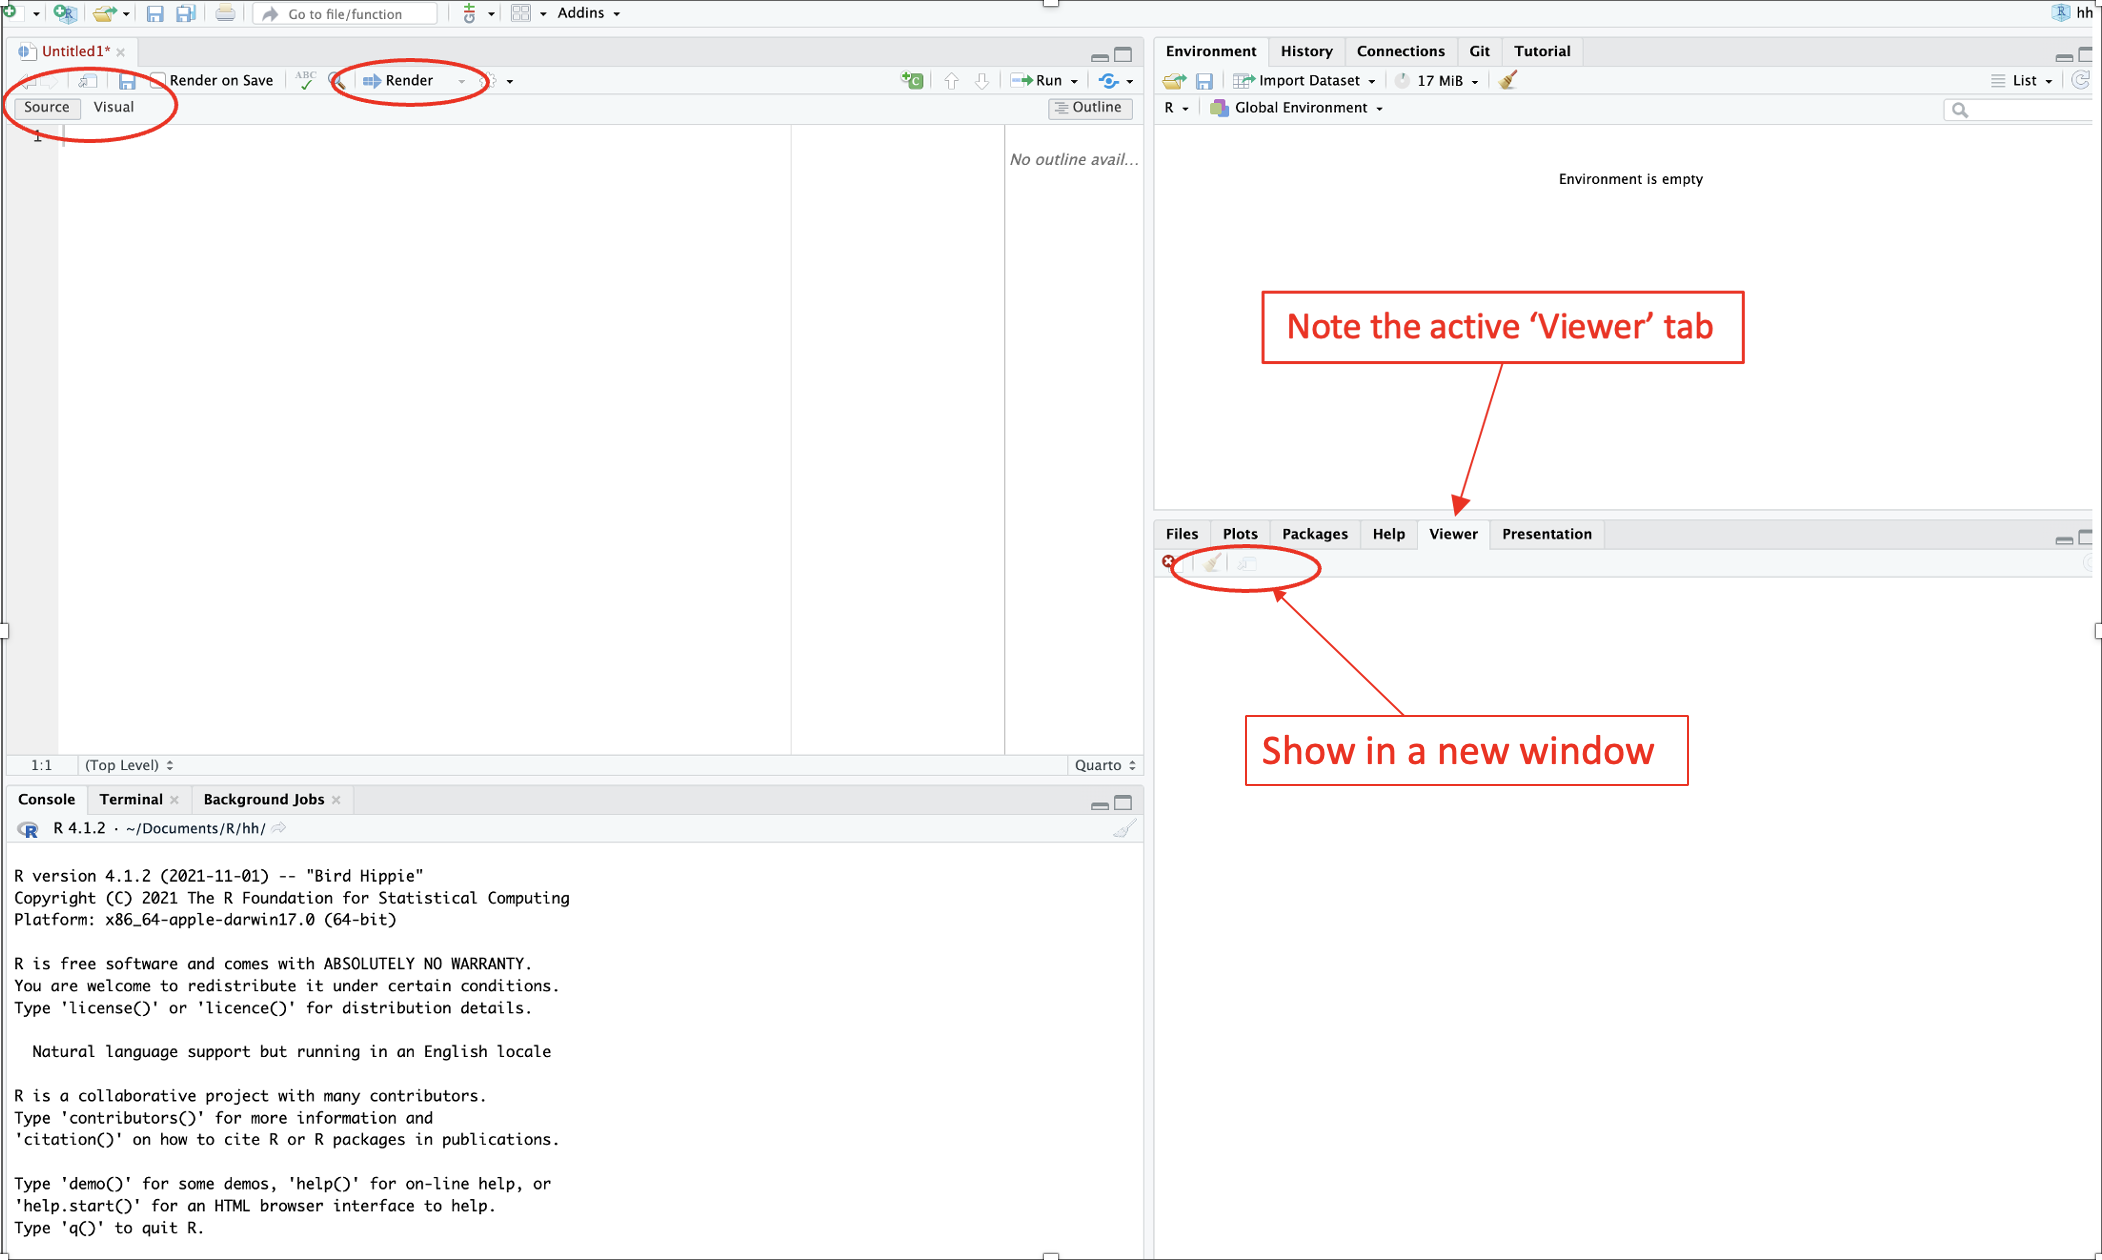
\includegraphics{/posts/rstudio-interf-2.png}
\end{block}

\begin{block}{Basics cont\ldots{}}
\phantomsection\label{basics-cont-2}
\begin{itemize}[<+->]
\tightlist
\item
  For a brief start-up, copy
  \href{https://github.com/usman-afzali/quarto-with-rstudio/blob/main/posts/quartoBasics.qmd}{this
  code} and paste it in the current open \texttt{.qmd} and hit render.
\item
  Alternatively, you can copy a similar \texttt{.qmd} document to the
  current project, open it, then edit and render it.
\item
  Demo
\item
  A comprehensive step-by-step tutorial is available on Quarto
  \href{https://quarto.org/docs/authoring/markdown-basics.html}{website}.
\item
  Or, you could watch this YouTube
  \href{https://www.youtube.com/watch?v=yvi5uXQMvu4}{video} in your own
  time. It is a bit outdated, but a great start.
\end{itemize}
\end{block}

\begin{block}{Add citations and reference list}
\phantomsection\label{add-citations-and-reference-list}
Best done using the \texttt{visual\ editor}.

E.g., Quarto can be used to create executable manuscripts in RStudio,
Python, or VS Code {[}@perkel2022{]}.
\end{block}

\begin{block}{Saving as pdf}
\phantomsection\label{saving-as-pdf}
Add the following code to \texttt{yaml}.

\begin{verbatim}
format:
  pdf:
    toc: true
    number-sections: true
    colorlinks: true
\end{verbatim}

Visit
\href{https://quarto.org/docs/output-formats/pdf-basics.html}{quarto
website} for further details.
\end{block}
\end{frame}

\begin{frame}[fragile]{Version control, Remote repositories, and
Blogging}
\phantomsection\label{version-control-remote-repositories-and-blogging}
\begin{block}{Git}
\phantomsection\label{git}

\includegraphics{/posts/git.png}

To know more: See
\href{https://www.git-scm.com/book/en/v2/Getting-Started-What-is-Git\%3F}{official
website}, or just this quick
\href{https://usman-afzali.github.io/quarto-with-rstudio/posts/git/git.html}{start-up
guide}
\end{block}

\begin{block}{GitHub}
\phantomsection\label{github}

\includegraphics{/posts/github.png}

\url{https://github.com}
\end{block}

\begin{block}{Blogging}
\phantomsection\label{blogging}
Now that we know basics of documentation, version control and remote
repos (I know, we are yet to demonstrate this), blogging is extremely
easy with Quarto. There are two ways:

\begin{enumerate}
\tightlist
\item
  We can add a \texttt{\_quarto.yml} file in to our local repo, render
  it, and it would starting shaping like a blog. This is the more
  complicated way.
\item
  We can use an available blog template, create a new local repo and
  take it from there.
\end{enumerate}

Here is a \href{https://youtu.be/YoKjBcuUP0s}{quick guide}.
\end{block}

\begin{block}{Blogging contd\ldots{}}
\phantomsection\label{blogging-contd}
Blogging with Quarto can be done with the use of Git and
\texttt{GitHub\ Pages}, or we can also use \texttt{PositCloud} instead
of GitHub Pages.

As we can see
\href{https://quarto.org/docs/publishing/github-pages.html\#render-to-docs}{here},
a must do step during blogging with GitHub Pages is rendering output
directory to \texttt{docs} in \texttt{\_quarto.yml}.

\begin{verbatim}
project:
  type: website
  output-dir: docs
\end{verbatim}
\end{block}

\begin{block}{Demo}
\phantomsection\label{demo}
Important steps for using remote repo are:

\begin{enumerate}
\tightlist
\item
  Installing Git
\item
  Creating a GitHub account
\item
  Connecting the local system with remote repo
\item
  Creating a repository on GitHub
\item
  Connecting the remote repo with the local one
\end{enumerate}

These steps are important whether or not we are blogging. For blogging,
then of course we need a publisher domain - which could be GitHub Pages
or PositCloud.
\end{block}
\end{frame}

\begin{frame}[fragile]{Quarto Templates}
\phantomsection\label{quarto-templates}
\begin{block}{An example}
\phantomsection\label{an-example}
\begin{itemize}
\tightlist
\item
  Taylor and Francis:
\end{itemize}

\url{https://github.com/mikemahoney218/quarto-tandf}.

Follow on-screen instruction.

\begin{itemize}
\tightlist
\item
  For further info, see
  \href{https://quarto.org/docs/journals/templates.html}{Article
  Templates}
\end{itemize}
\end{block}

\begin{block}{Advantages of documentation with Quarto}
\phantomsection\label{advantages-of-documentation-with-quarto}
\begin{itemize}
\tightlist
\item
  Keep your data files and write up files integrated.
\item
  Create re-usable workflow -- becomes much easier once we are familiar.
\item
  Use version control to see the previous versions.
\item
  Hide/show \texttt{R} code when appropriate.
\item
  Move ready-made \texttt{.qmd} files to a journal template rather than
  re-formatting the whole manuscript.
\item
  The pdf version is generally appropriate for \texttt{PsyArXiv}.
\end{itemize}
\end{block}
\end{frame}

\begin{frame}[fragile]{Presentation}
\phantomsection\label{presentation}
\begin{block}{Basic slides}
\phantomsection\label{basic-slides}
\begin{itemize}
\tightlist
\item
  We used the good ol' \texttt{.qmd}.
\item
  Add \texttt{revealjs} in the format. Or, to make it more elaborate:
\end{itemize}

\begin{verbatim}
format: 
  revealjs:
    theme: simple
    highlight-style: github
    slide-number: c/t
\end{verbatim}

\begin{itemize}
\item
  Further info: \url{https://quarto.org/docs/presentations/}
\item
  Demo: let's use the current slides as an example :)
\end{itemize}
\end{block}

\begin{block}{Sharing slides}
\phantomsection\label{sharing-slides}
\begin{enumerate}
\tightlist
\item
  Save as pdf: This option only works with \texttt{Google\ Chrome} as
  explained
  \href{https://quarto.org/docs/presentations/revealjs/presenting.html\#print-to-pdf}{here}.
  Or, see below. 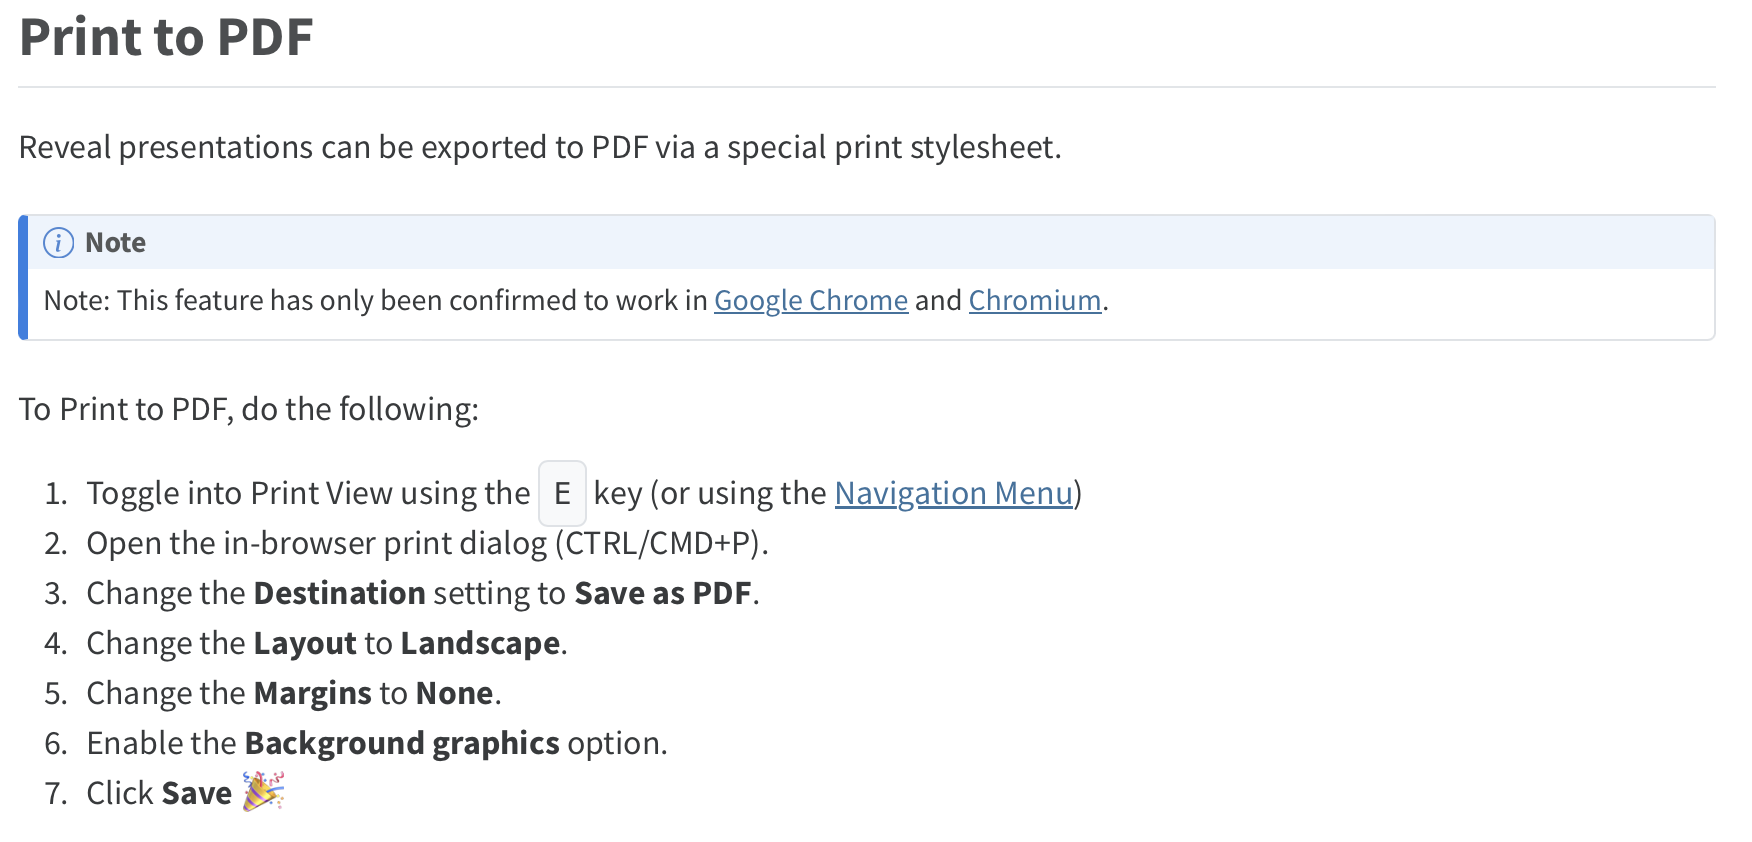
\includegraphics{/posts/pdf.png}
\end{enumerate}
\end{block}

\begin{block}{Sharing slides}
\phantomsection\label{sharing-slides-1}
\begin{enumerate}
\setcounter{enumi}{1}
\tightlist
\item
  Provide the url from the blog/site.
\end{enumerate}

What are the advantages?
\end{block}

\begin{block}{Final thoughts}
\phantomsection\label{final-thoughts}
\begin{itemize}
\item
  How I use Quarto: See my
  \href{https://github.com/usman-afzali?tab=repositories}{repositories}
\item
  Getting Help:
  \href{https://github.com/mcanouil/awesome-quarto}{Awesome Quarto},
  Quarto website, YouTube, social media.
\item
  Anonymous feedback: please use this
  \href{https://forms.gle/w4dp1UgRGZ3Vbgqf8}{link}
\end{itemize}
\end{block}

\begin{block}{Karakia Whakatūwhera}
\phantomsection\label{karakia-whakatux16bwhera-1}
\begin{figure}

\begin{minipage}{0.50\linewidth}
Unuhia, unuhia/ Te pou, te pou/ Kia wātea, kia wātea/ Āe, kua
wātea\end{minipage}%
%
\begin{minipage}{0.50\linewidth}
Remove, uplift/ The posts/ In order to be free/ Yes, it has been
cleared/\end{minipage}%

\end{figure}%
\end{block}
\end{frame}

\begin{frame}{THE END}
\phantomsection\label{the-end}
\end{frame}

\begin{frame}{References}
\phantomsection\label{references}
\end{frame}



\end{document}
